\subsection{Software}
Im folgenden wird die Ansteuerung und Auswertung der elektrischen Komponenten näher beschrieben. Außerdem wird die Kommunikation zwischen der Host- und Target-Plattform erläutert. Als Zielplattform wird ein BeableBoneBlack verwendet, auf welchem eine Linux-Distribution ausgeführt wird. In der folgenden Abbildung sind die einzelnen Bausteine und deren Verbindung zu der Zielplattform dargestellt.

\begin{figure}[!h]
\centering
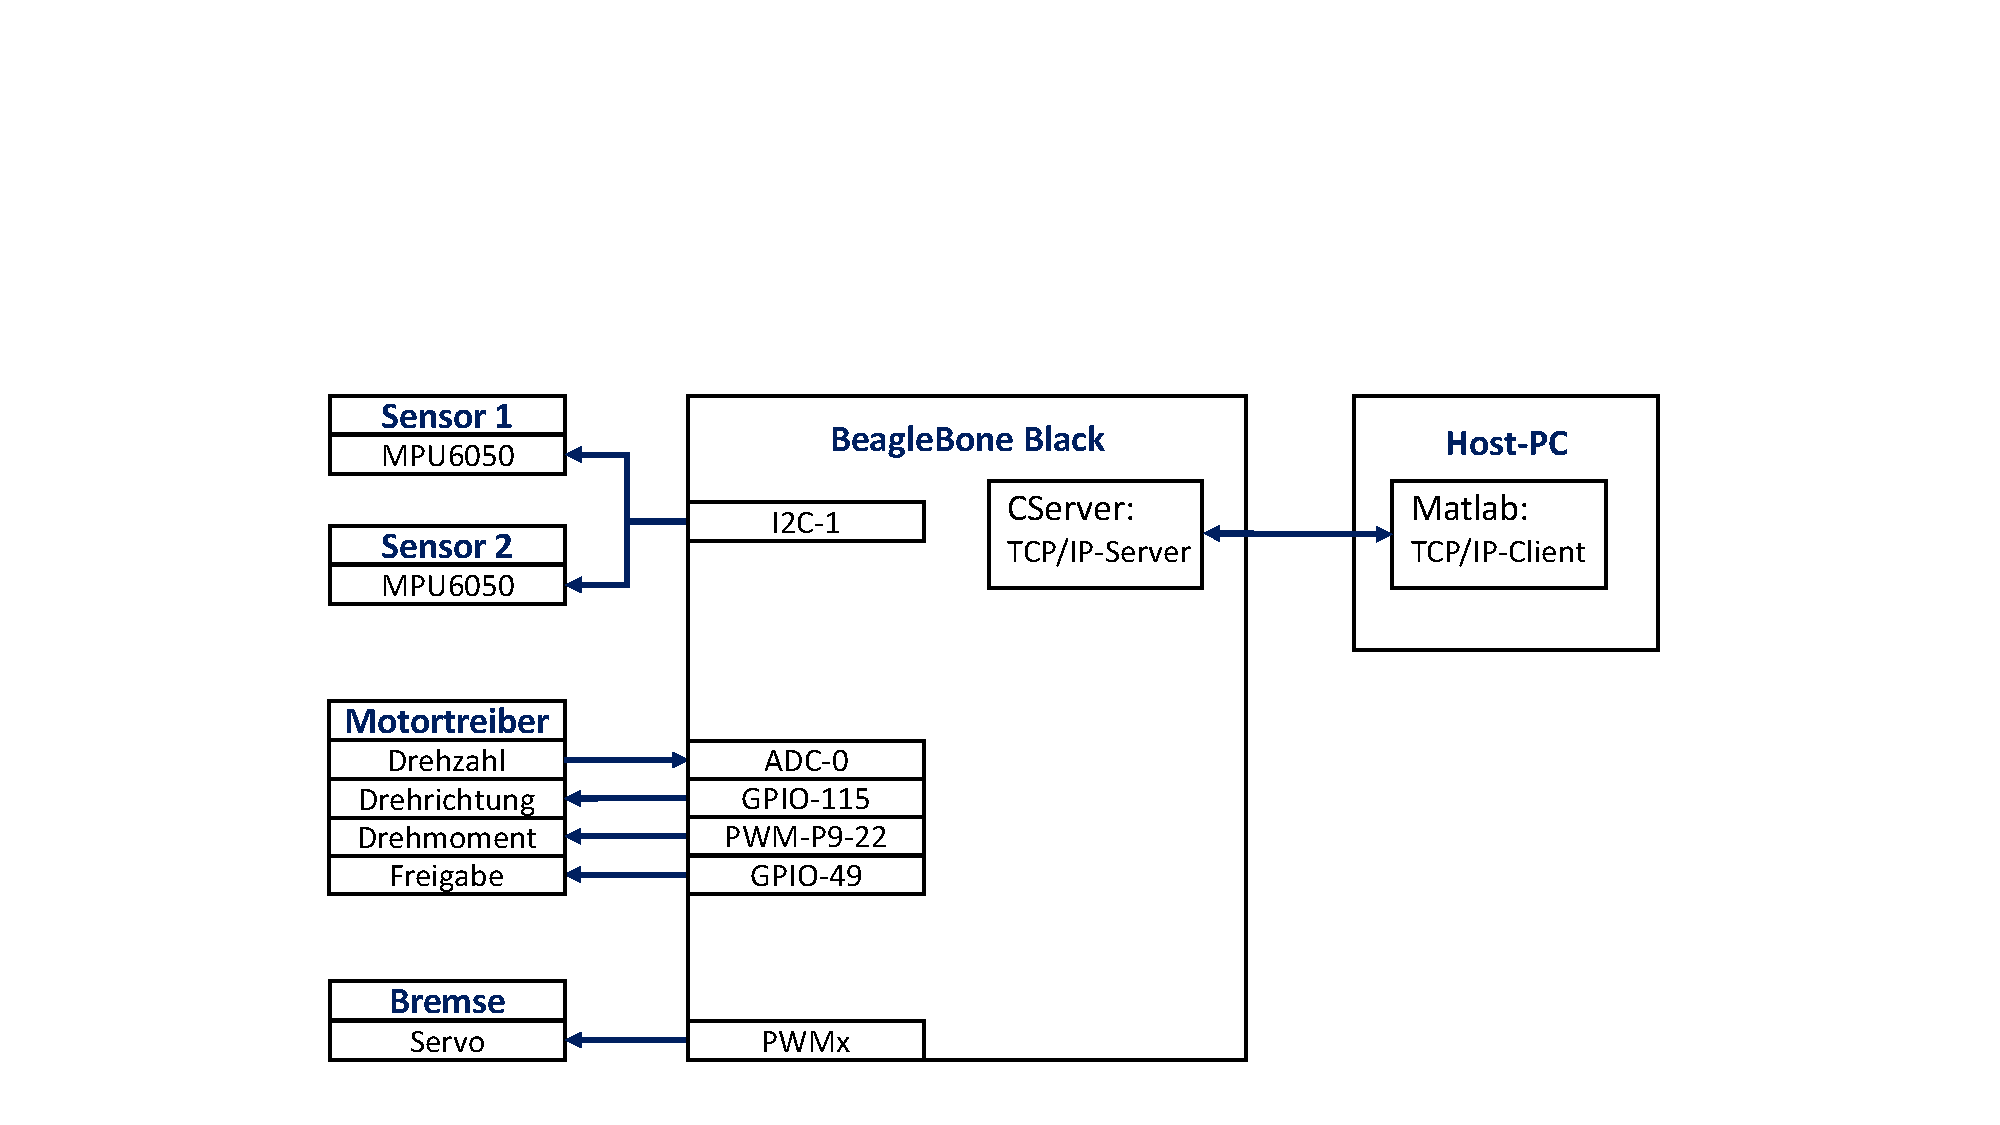
\includegraphics[width=0.8\linewidth, trim={4cm 1cm 5cm 6cm},clip]{img/ElekAufbau_Kommunikation}
\caption{Blockschaltbild der Komponenten, Quelle: eigene Darstellung}
\end{figure}

Die Interaktion mit den Treibern des Betriebssystems wird mit Hilfe von Klassen gekapselt. Dadurch entsteht eine einheitliche und benutzerfreundliche Schnittstelle zwischen Hard- und Software.